\documentclass{elsarticle}


\usepackage[utf8]{inputenc}    % utf8 support       
\usepackage{amsmath,amssymb, amsthm,mathtools,mathrsfs,stmaryrd,titletoc}


% bibtex 
\usepackage{natbib}



\usepackage[retainorgcmds]{IEEEtrantools}
\usepackage[usenames]{color}
\usepackage{tabularx}
\usepackage{booktabs}
\usepackage[font=small,labelfont=md]{caption,subfig}
\usepackage{multirow}
\usepackage[bookmarks=true,colorlinks=true,linkcolor=blue,citecolor=red,backref=page]{hyperref}


\usepackage{mathtools}

\definecolor{darkgray}{rgb}{0.95,0.95,0.95} % color used in tables

\newcommand{\bfsigma}{\boldsymbol{\sigma}}
\newcommand{\bfepsilon}{\boldsymbol{\epsilon}}
\newcommand{\bfu}{\boldsymbol{u}}
\newcommand{\bfx}{\boldsymbol{x}}
\newcommand{\bfphi}{\boldsymbol{\phi}}
\newcommand{\bftheta}{\boldsymbol{\theta}}
\newcommand{\te}{\text{e}}
\newcommand{\td}{\text{d}}
\newcommand{\tp}{\text{p}}
%-----------------------------------------------------------------------
\newcommand{\tty}[1]{\textnormal{\texttt{#1}}}
\newcommand{\sym}[1]{\textnormal{\textit{#1}}}
\newcommand{\eg}{\textit{e.g.}\xspace}
\newcommand{\ie}{\textit{i.e.},\xspace}
\newcommand{\etc}{\textit{etc.}\@\xspace}
\newcommand{\vm}[1]{\mathbf{#1}}
\newcommand{\trans}{^\mathrm{T}}
\newcommand{\bsym}[1]{\boldsymbol{#1}}

\begin{document}

%\newcommand\barbelow[1]{\stackunder[1.2pt]{$#1$}{\rule{.8ex}{.075ex}}}

\begin{frontmatter}



%\title{Modeling crack propagation of concrete gravity dams with the phase-field regularized cohesive zone model}
\title{\textbf{How to effortlessly write a high quality scientific paper in the field of computational engineering and sciences }}

%\tnotetext[label1]{Dedicate to }

% use optional labels to link authors explicitly to addresses:
% \author[label1,label2]{}
% \address[label1]{}
% \address[label2]{}

\author[1]{Vinh Phu Nguyen\corref{cor1}}
 \ead{phu.nguyen@monash.edu}
\author[2]{Stephane Bordas}
\author[3]{Alban de Vaucorbeil}

\cortext[cor1]{Corresponding Author}

\address[1]{Department of Civil Engineering, Monash University, Clayton 3800, VIC, Australia}
\address[2]{Institute of Computational Engineering, University of Luxembourg, Faculty of Sciences Communication and Technology, Luxembourg}
\address[3]{Institute for Frontier Materials, Deakin University, Geelong, VIC, 3216, Australia}
%\maketitle


%\pagestyle{fancyplain}
%\pagenumbering{arabic}

\begin{abstract}
Starting with a working good research idea, this paper outlines a scientific writing process that helps us to have a nearly complete paper when the last analysis task has been finished.  The key ideas of this process are: (1) writing should start early in the research project, (2) research and writing are carried out simultaneously, (3) best tools for writing should be used.  The process seems working well as it has helped us writing thousands of pages without feeling a pain. We hope it works for you too.  Due to our personal preferences, the discussion is confined to \LaTeX\ based typesetting where we present guidelines to prepare high-quality images, tables, algorithms and source codes using \LaTeX. We also discuss writing guidelines such as paper structure and some common mistakes.
\end{abstract}

% *********************************************************************************************************

\begin{keyword}
 scientific writing; \LaTeX; scientific publication; high quality writing.
\end{keyword}

\end{frontmatter}

\tableofcontents

%%%%%%%%%%%%%%%%%%%%%%%%%%%%%%%
\section{Introduction}

\begin{table}[h!]
      \centering
      \caption{Summary statistics of the use of \LaTeX\ in science disciplines (\% of submitted papers) taken from \url{https://www.the-scientist.com/uncategorized/dont-format-manuscripts-44040}.}
      \setlength\fboxsep{0pt}
      \vskip-\topsep%
      \smallskip%
      \renewcommand\arraystretch{1.4}
      \colorbox{darkgray}{%
      \begin{tabularx}{0.5\textwidth}{ll}
      \toprule
       Disciplines & \LaTeX\ rate \\
      \midrule
       Mathematics & 96.9\% \\
       Statistic and Probability & 89.1\% \\
       Physics & 74.0\%\\
       Computer Sciences & 45.8\%\\
       Engineering & 1.0\%\\
       \bottomrule
       \end{tabularx}%
      }
      \label{table:latex}
      \end{table}
      
      where is my equation? 
\begin{equation}
  \mathscr{E} (\bfu, d) 
    = \int_{\varOmega_{0}} \left[\omega(d)\psi_{0}^+(\bfepsilon (\bfu)) + \psi_{0}^-(\bfepsilon (\bfu)) \right]\td V
    + \int_{\varOmega_{0}}  \frac{G_\text{f}}{c_\alpha} \left[ \frac{1}{b} \alpha(d)
    + b \left( \nabla d \cdot \nabla d \right) \right] \td V
    - \mathscr{P} (\bfu) + \beta  
\label{eq:3}
\end{equation}

\begin{figure}[!h]
  \centering
  \subfloat[\texttt{Illustrator} and \texttt{LaTeXiT}]{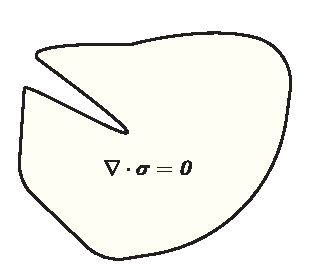
\includegraphics{Taylor-bar-setup}\label{fig:figures11a}}
  \subfloat[\texttt{Inkscape} and PDF\_TEX]{\input{Taylor-bar-setup_pdf_tex.pdf_tex}\label{fig:figures11b}}
  \caption{Using \texttt{Illustrator} and \texttt{Inskcape} to produce vector images with \LaTeX\ symbols. The font in figure (a) is slightly different from the one in the text ($\nabla\cdot\boldsymbol{\sigma} = \boldsymbol{\mathit{0}}$), while it matches perfectly in figure (b).}
  \label{fig:figures11}
\end{figure}
      
\end{document}